\chapter{The Neural Engineering Framework}\label{sec:nef}

To construct a large-scale spiking neural network with a certain behaviour, some method for obtaining that behaviour is required.
In most cases this method will be a learning algorithm \parencite[e.g.,][]{oreilly2006}.
However, this requires time-intensive training of the model and is often not viable for large models, complex behaviours, or models combining different behaviours.
In this work I opt to use the Neural Engineering Framework \parencite[NEF;][]{eliasmith2003} which allows the direct construction of a spiking neural network from the mathematical equations describing the desired dynamics without the time-intensive training.
As such the final model does not provide an developmental account of how the neural network became organized or learned to perform its task.
But, it provides a biologically plausible explanation of how the developed brain might perform that task.
As well, it allows for the inclusion of biologically plausible online learning rules, to test adaptation in the adult system.
Furthermore, it allows for manipulations to test known experimental results in the model or obtain new predictions.
The NEF consists out of the three core principles for \emph{representation}, \emph{transformation}, and \emph{dynamics} in a neural network that I introduce in this order.

\section{Representation}
Neurons within a neural network will have a preferred stimulus: they will fire most strongly for that stimulus and less strongly as the stimulus gets more dissimilar to the preferred stimulus (see \cref{fig:tuningcurve}).
To capture this in a mathematical description, we can treat the stimulus as a vector $\vc x(t)$ that varies over time.
The preferred stimulus vector, that is the vector a neuron $i$ fires most strongly for, will be denoted with $\enc_i$.
The spiking activity $\act_i(t)$ of a neuron can then be described with
\begin{equation}
    \act_i(t) = \nl\!\sbr{\gain_i \langle\enc_i, \vc x(t)\rangle + \jbias_i}
\end{equation}
where $\gain_i$ is a neuron gain factor, $\jbias_i$ a bias input current, and $\nl$ the neuron nonlinearity.
The nonlinearity $\nl$ represents the neuron model and converts an input current into spikes.
Usually this is the spiking, leaky integrate-and-fire model (LIF) discussed in \cref{sec:neurons}, which provides a good trade-off of captured neuron behaviour, detail, and simulation effort.
But simpler neuron models (e.g., a rate-based LIF model, or rectified linear units) could be used, as well as much more complex neuron models, like the compartmental models in \textcite{eliasmith2016} and \textcite{duggins2017c}.
The input current to the neuron is obtained from how well the stimulus aligns with the preferred stimulus as measured by the dot product.
As this alignment with the preferred stimulus ``encodes'' the stimulus into the neural representational space, $\enc_i$ is usually referred to as \emph{encoder} in the context of the NEF\@.
Furthermore, the gain factor $\gain_i$ and bias term $\jbias_i$ can be used to adjust the neuron's tuning curve to experimentally observed firing rates.
However, it is also common to use higher maximal firing rates to use fewer neurons in simulations while achieving an similar accuracy.
While this is not entirely adhering to biological constraints, in most cases NEF models behave similarly when lowering the firing rates and increasing neuron numbers accordingly \parencite[e.g.,][]{gosmann2015}.
As it is rare to have detailed information about the tuning curves in many parts of the brain, those values are usually not directly set in the NEF\@.
Instead a representational space $\repspace$ is defined, usually as the $\dims$-dimensional hyperball with radius $\radius$.
Furthermore, for each neuron a maximum firing rate $\act_{\max, i}$ and an intercept point $p_i$ are sampled from random distributions.
These values are used to calculate the gain and bias so that the neuron starts firing at $p_i \enc_i$ when $\vc x$ varies along the encoder $\enc_i$ and that the maximum $\act_{\max,i}$ is not exceeded across the representational space $\repspace$.
\begin{figure}
    \begin{captionbeside}[A typical neuron tuning curve.]{A typical neuron tuning curve. The thick black line shows the mean firing rate in dependence of a stimulus parameter (e.g., rotation of a bar). The thin blue lines show the standard deviation. Figure reproduced from \textcite{butts2006} and reused under the Creative Commons Attribution license.\label{fig:tuningcurve}}[l]
        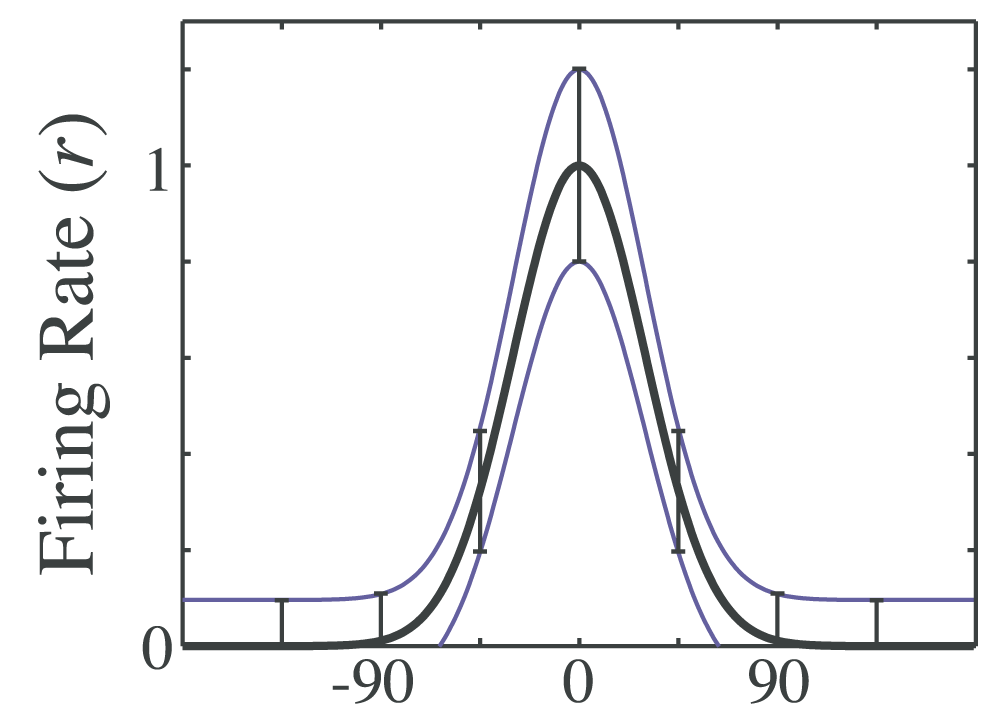
\includegraphics[scale=1.3]{figures/tuningcurve}
    \end{captionbeside}
\end{figure}

Given a population of neurons, also called a neural \emph{ensemble} in NEF terms, how can the encoded vector $\vc x(t)$ be recovered?
First the activity or spike trains $\act_i(t)$ are convolved with a synaptic filter $\syn$ to obtain the induced post-synaptic voltage change.
Usually this is a decaying exponential
\begin{equation}
    \syn(t) = \syntau^{-1}\exp\!\big({-t} / \syntau\big) \text{,}
\end{equation}
but other filters can be used to more precisely model the dynamics of the synapse \parencite{voelker2017a} and even extensions to conductance-based synapses are possible \parencite{stockel2017}.
From the filtered activity, the represented vector can be reconstructed with a linear, weighted decoding
\begin{equation}
    \hat{\vc x}(t) = \sum_i \dec_i \cdot \sbr{a_i * h}\!(t)
\end{equation}
with decoding weights $\dec_i$.

To get a good reconstruction of the represented value, the decoding weights should minimize the error
\begin{equation}
    E = \int_{\repspace} \norm{\vc x - \hat{\vc x}}^2 \dif \vc x \text{.}
\end{equation}
In general, this minimization cannot be solved analytically.
Thus, in the NEF the integral is approximated by randomly sampling $M$ \emph{evaluation points} $\evalp_k \in \repspace$.
Given the finite number of evaluation points, it becomes possible to solve for the decoding weights with a least-squares minimization.
The detailed derivation is given in \textcite[Ch.~2]{eliasmith2003}.
In short, one obtains the matrices
\begin{equation}
    \actmat = \sbr{\begin{array}{cccc}
            \act_1(\vc x_1) & \act_1(\vc x_2) & \cdots & \act_1(\vc x_M) \\
            \act_2(\vc x_1) & \act_2(\vc x_2) & \cdots & \act_2(\vc x_M) \\
            \vdots & \vdots & \ddots & \vdots \\
            \act_N(\vc x_1) & \act_N(\vc x_2) & \cdots & \act_N(\vc x_M) \\
    \end{array}}
    \ \text{and}\ 
    \evalpmat = \sbr{\begin{array}{c}
            \vc x_1 \\ \vc x_2 \\ \vdots \\ \vc x_M
    \end{array}}
\end{equation}
where one can use the steady-state activities in the activity matrix $\actmat$ which can be obtained analytically for LIF neurons.
Given these two matrices the decoding weights can be obtained with the regularized pseudo-inverse as
\begin{equation}
    \sbr{\begin{array}{c}
            \dec_1\Tr \\ \dec_2\Tr \\ \vdots \\ \dec_N\Tr
        \end{array}} = \del{\actmat \actmat\Tr + M \reg^2 {\max(\actmat)}^2 \imat}^{-1} \actmat \evalpmat
\end{equation}
where $\reg$ is the regularization scale (usually $\reg = 0.1$).

The encoders and decoders not only allow us to encode information into a neural ensemble and decode it back out, but also to transmit that information from one neural population to another.
By decoding from the pre-synaptic ensemble and encoding into the post-synaptic ensemble, the connection weights required between the two populations can be obtained as
\begin{equation}
    \weights_{ij} = \enc_i\Tr \mat T \dec_j
\end{equation}
where $\mat T$ can describe a linear transform to implement across the neural connections.
If $\mat T$ is the identity matrix, the connection will be a pure communication channel.


\section{Transformation}
To be useful, a neural network has to transform or compute functions on the represented information.
In the NEF, it is straight-forward to implement a given transformation in the connection weights between two ensembles.
To implement a function $f(\vc x)$, one replaces the matrix $\evalpmat$ with
\begin{equation}
    \evalpmat_{f(\vc x)} = \sbr{\begin{array}{c}
            f(\vc x_1) \\ f(\vc x_2) \\ \vdots \\ f(\vc x_M)
    \end{array}}
\end{equation}
when solving for decoders.
This corresponds to a minimization of the modified error $E_{f(\vc x)} = \int_{\repspace} \norm{f(\vc x) - \hat{\vc x}}^2 \dif \vc x$.

\Textcite[Ch.~7]{eliasmith2003} shows that a neural network constructed in this way is typically best at computing low-order polynomials.
Non-smooth or discontinuous functions might require a large number of neurons.
In some cases a better function approximation can be achieved by appropriately selecting parameters like intercepts or encoders or by changing the network structure to decompose a function in a different way.
An example is the calculation of products and has been discussed in \textcite{gosmann2015-1}, and \cref{sec:thresholding} shows this for the thresholding of values.

\section{Dynamics}
The final principle of the NEF addresses dynamics.
In linear control theory a dynamical system is often described by state equations of the form
\begin{align}
    \od{\vc x}{t} &= \mat A \vc x(t) + \mat B \vc u(t) \label{eqn:statespace1} \\
    \vc y(t) &= \mat C \vc x(t) + \mat D \vc u(t) \label{eqn:statespace2}
\end{align}
where $\vc x(t)$ is the state vector, $\vc u(t)$ the input vector, and $\vc y(t)$ the output vector.
The system behaviour is determined by the dynamics matrix $\mat A$, input matrix $\mat B$, output matrix $\mat C$, and the feedthrough matrix $\mat D$.
\Cref{fig:statespace} shows a graphical representation.
\begin{figure}
    \centering
    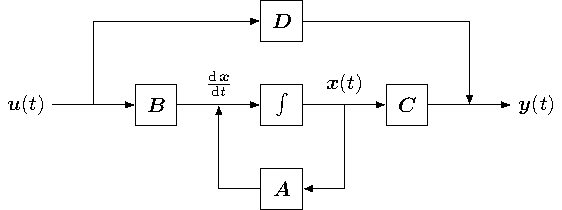
\includegraphics{tikz/statespace}
    \caption{Visualization of \cref{eqn:statespace1,eqn:statespace2} as block diagram.}\label{fig:statespace}
\end{figure}

In the NEF, we want to map a given dynamical system onto neural components (\cref{fig:neural-lti}).
The neuron dynamics are dominated by the synaptic filter \parencite[Appendix~F.1]{eliasmith2003} which becomes the transfer function and gives
\begin{equation}
    \vc x(t) = \syn(t) * \sbr{\mat A' \vc x(t) + \mat B' \vc u(t)} \text{.}
\end{equation}
With help of the Laplace transform one can obtain $\mat A'$ and $\mat B'$ from $\mat A$ and $\mat B$ as
\begin{align}
    \mat A' &= \syntau \mat A + \imat \\
    \mat B' &= \syntau \mat B  \text{.}
\end{align}
This implies that to implement a dynamical system with a neural ensemble, the input has to be multiplied by $\syntau$ to account for the synaptic filtering.
In addition, one needs to add a recurrent connection implementing the function $f(\vc x) = \syntau \mat A \vc x + \vc x$.
Note that combining this third principle with the principle of transfomation, allows the implementation of nonlinear dynamics in a spiking neural network.
\begin{figure}
    \centering
    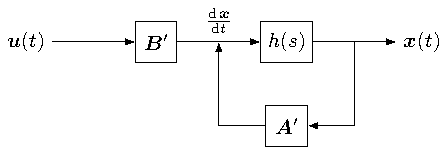
\includegraphics{tikz/neural-lti}
    \caption[Block diagram of the linear system of a neural population.]{Block diagram of the linear system of a neural population. $h(s)$ is the Laplace transformed synaptic filter $\syn(t)$.}\label{fig:neural-lti}
\end{figure}


\section{Simulating NEF networks}
To simulate NEF style networks, I use the Python library Nengo \parencite{bekolay2014,sharma2016}.
It supports different backends to run neural models on different hardware platforms.
For example, Nengo OCL targets GPUs with an OpenCL implementation.
While this allows better simulation performance, special case implementations are necessary for certain features.
In particular, this applies to the association matrix learning rule (see \cref{sec:aml}).
Moreover, I utilized the Sharcnet and Compute Canada high-performance clusters which typically provide more CPU resources than GPU resources.
Thus, I mostly used the Nengo reference (CPU) backend.
To obtain sufficient simulation performance for the size of models constructed in this work, it was necessary to optimize memory organization of the internal data structures of the backend.
While the exact details are out of the scope of this thesis, they are published in \textcite{gosmann2017}.
